\chapter{Outlook}\label{ch:outlook}

The results of the experiments in chapter \ref{ch:experiments} show, that machine learning algorithms can indeed predict the stock price change based on a business report.
The presented results have however some problems that should be considered.
The first thing that is problematic is, that trading fees of the stock exchanges were not taken into account.
That means that even if the classifier correctly predicts a positive price change, there is still a chance, that the total return is negative, if the fees exceed the stock price gains.
Another issue is, that the classifiers only make assumptions about a time span of two days, which is just a small fraction of all trading days in a year.
Therefore all losses within these two days can be compensated during the remaining year and, vice versa, all gains in this small time span can be lost again in the following period.
To determine whether the algorithms cound also be used in a long-term scenario, it would be necessary to run a simulation in which stocks are bought based on the classification results.
A possible simulation that test how well the short-term prediction works during one year is depicted by the flowchart in figure \ref{figure:long_term_simulation}.
\begin{figure}[h]
    \centering
    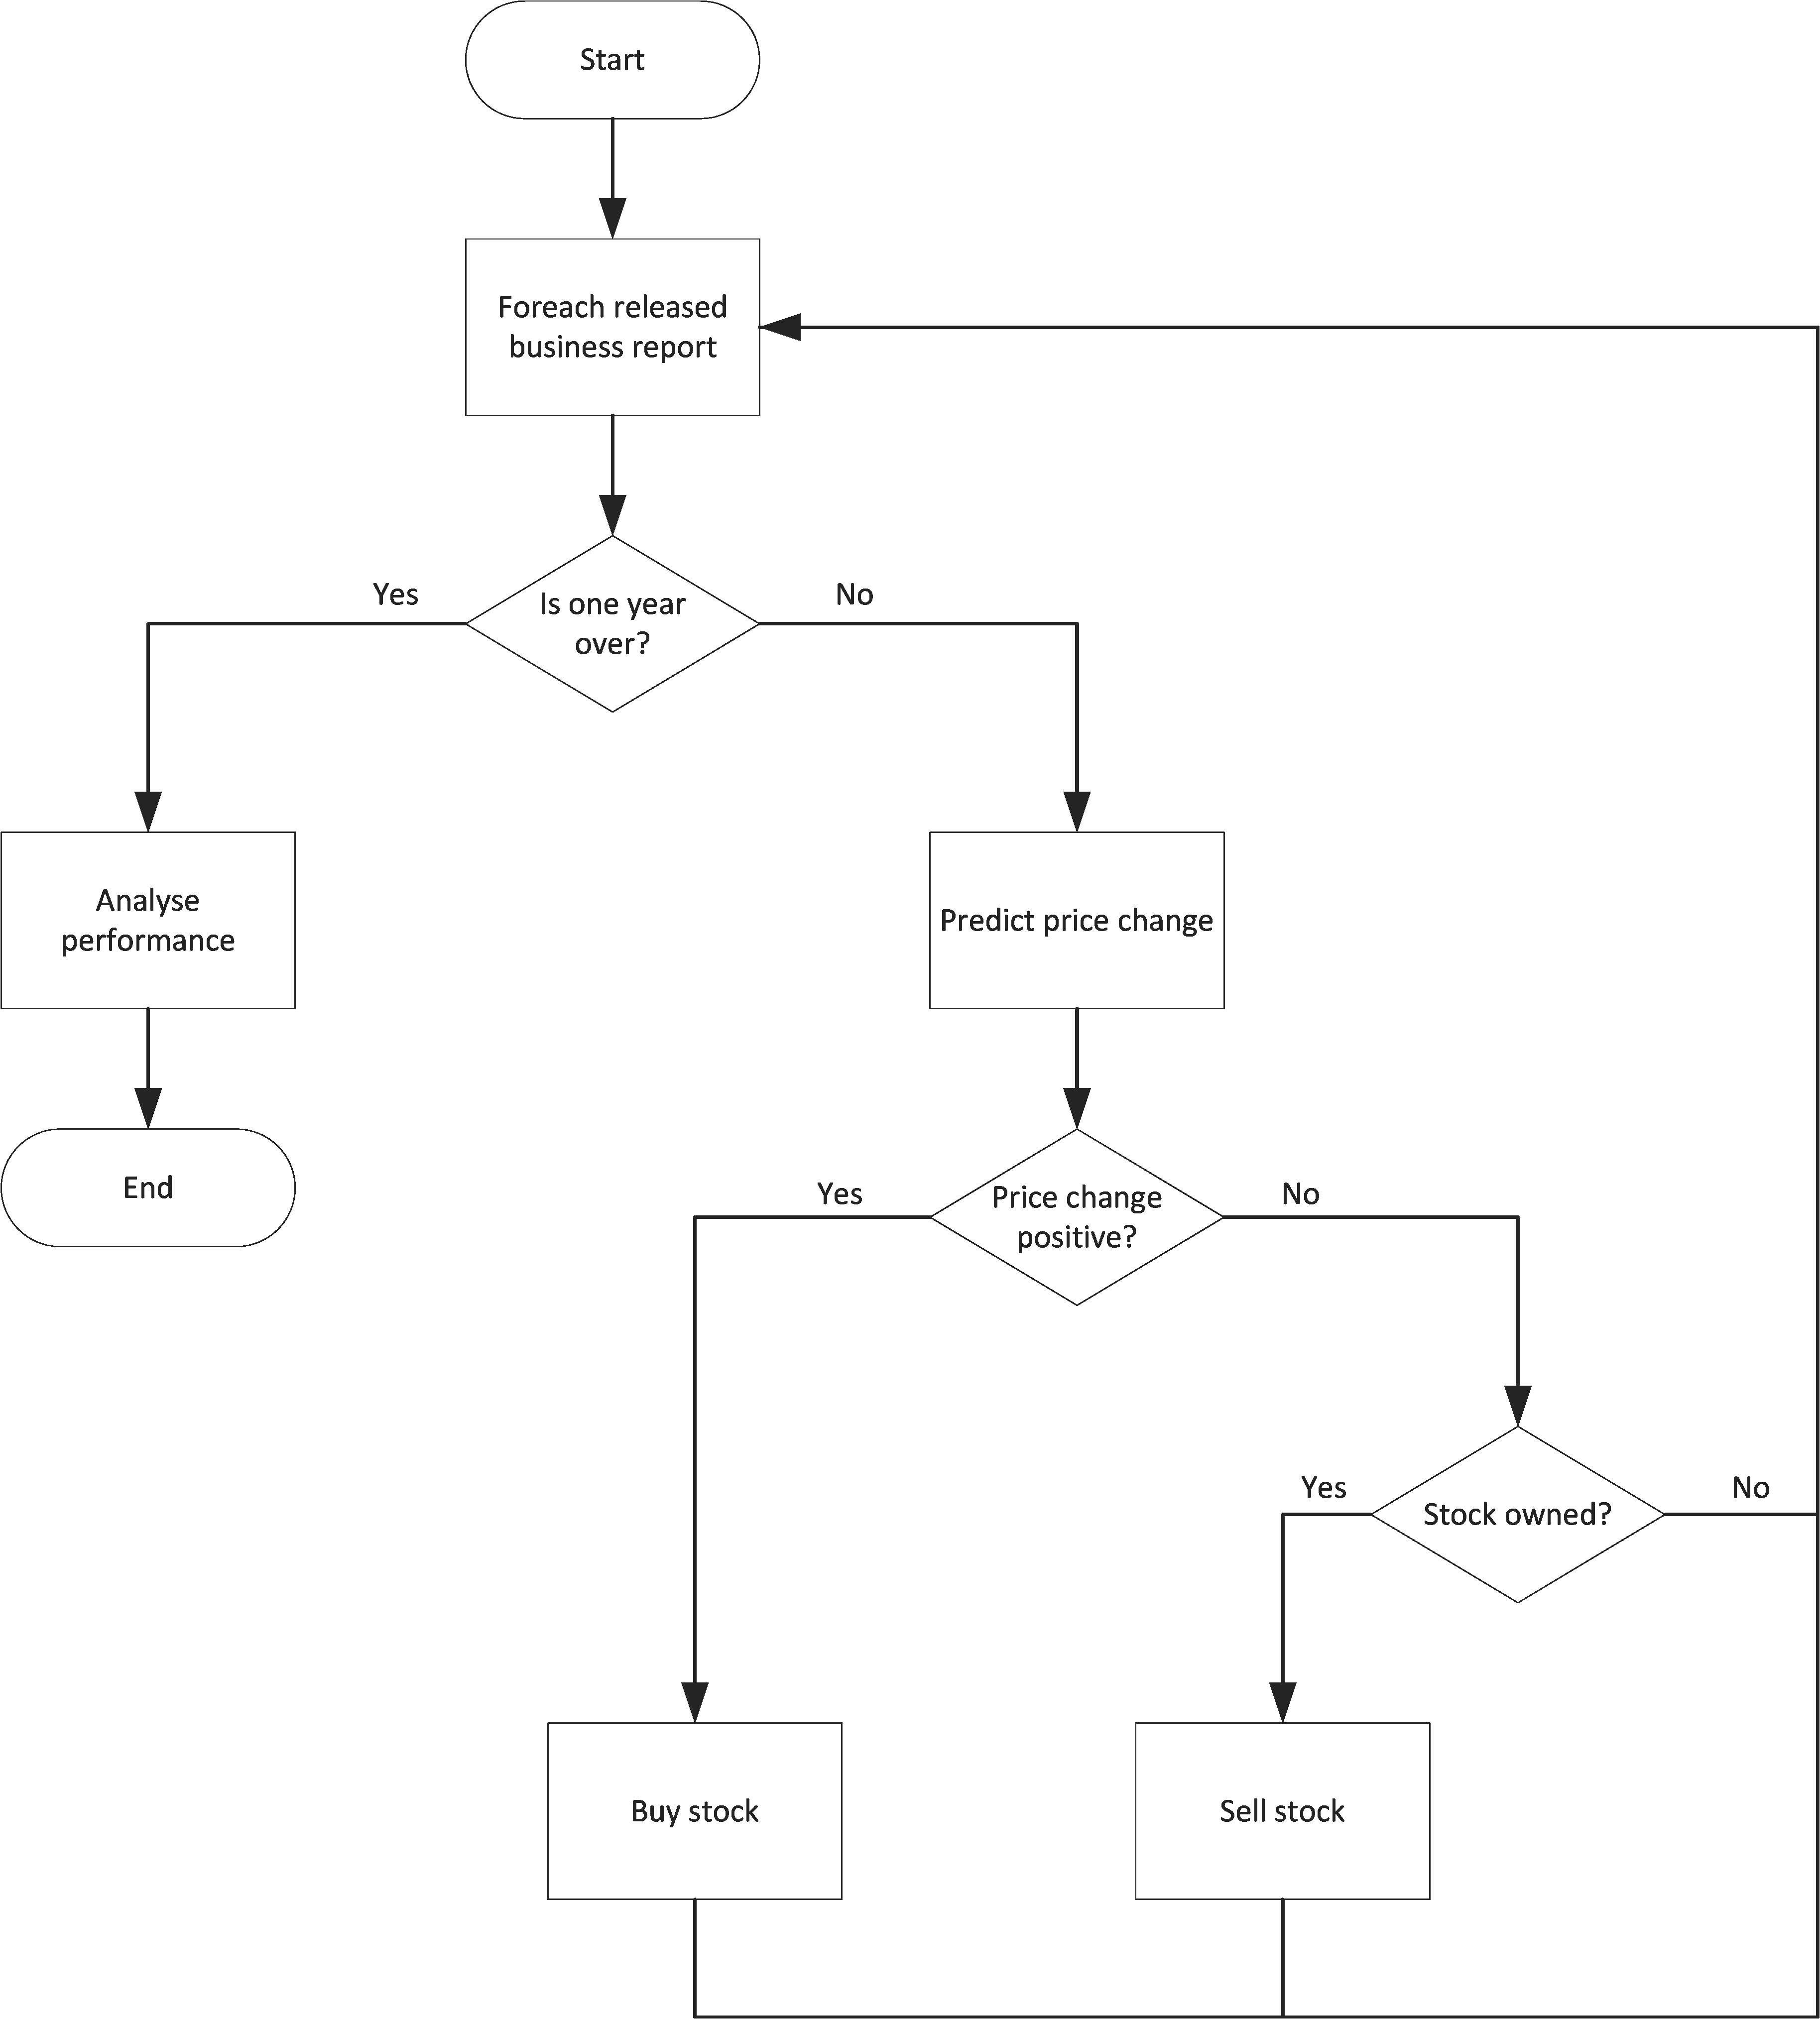
\includegraphics[width=\textwidth]{figures/Simulation.png}
    \caption{A possible simulation that tests how well the short-term prediction work in a long-term scenario.}
    \label{figure:long_term_simulation}
\end{figure}
% In general the introduced algorithms could be described as short-term speculating agents, which speculate on rising or falling stock prices in the next two days from the report release day.

A more sophisticated approach would be to immediately predict the price change for a longer time.
The aim could be for example, to predict the stock price change ratio for the next five years, based on business reports from the past five years.
This could be realised with a \ac{LSTM} with the document embeddings as the timesteps.
This scenario would also be more similar to the work of an investor who holds shares for a long period.
A way to improve the prediction accuracy, whould be to also use the business figures, like profit or equity, as input features to the classifiers.
Since common business valuation methods use these figures, the stock price is heavily influenced by them.
The classifiers should therefore also benefit from having this information available.
% has a practical usage, a longer test with a play portfolio would be necessary, for which no time was available.


% There are however a few indices, that the algorithms would perform worse than most investors and would probably even lose all money invested.
% The first thing that is problematic is, that trading fees of the stock exchanges were not taken into account.
% That means that even if the classifier correctly predicts a positive price change, there is still a chance, that the total return is negative.
% Another issue is that the classifier bases its decisions only on one report, whereas an investor would typically evaluate the reports of multiple years.
% In general the introduced algorithm could be described as a short-term speculating agent, which speculates on rising or falling stock prices in the next two days from the report release day.
% However it would be interesting how well such a machine learning algorithm performs in a more long-term scenario, using business reports from the last ten years and predicting the stock price change in ten years.
% This could also be realised with a \ac{LSTM}, which would be trained with the business reports of the past ten years from the newest report and the change ratio for the next ten years as the label.
% This scenario would also be more similar to the work of an investor who holds shares for a long period.
% A way to improve the prediction accuracy, whould be to also use the business figures, like profit or equity, as input features to the classifiers.
% Since common business valuation methods use these figures, the stock price is heavily influenced by them.
% The classifiers should therefore also benefit from having this information available.

There is also another limitation, that would have to be solved before the software could be used in a practical application:
At the moment, the data preprocessing, feature extraction and classification step are all started manually when they are needed.
For a practical application they would have to be started by a script one after another and each step should ideally not write its results to a file but pass it to the next script as a parameter.

% This could lead to the behaviour, that the algorithm would predict a positive price change, based on a single positive quarterly report

